% Declare type of document
\documentclass[10pt]{article}

% Import Packages
\usepackage[utf8]{inputenc} 

% Commonly used math symbols and fonts
\usepackage[mathscr]{euscript}
\usepackage{amsfonts,amsmath,amssymb,amsthm}
\usepackage{mathtools,mathdots}

% Better looking default font
\usepackage{lmodern}

% itemize environment
\usepackage{enumitem}
\usepackage{enumerate}

% Array, longtable, and booktabs
\usepackage{array}
\usepackage{longtable}
\usepackage{booktabs}
 
% Caption package for hiding Figure #
\usepackage{caption}

% Page formatting
\usepackage[letterpaper, margin=1in]{geometry}

% Package for nice syntax highlighting for code
% \usepackage[cache=false]{minted}
\usepackage{minted} 

% Allows line breaks in the math environment
\allowdisplaybreaks

\usepackage[activate={true,nocompatibility},final,tracking=true,kerning=true,spacing=true,factor=1100,stretch=10,shrink=10]{microtype}
\microtypecontext{spacing=nonfrench}
% activate={true,nocompatibility} - activate protrusion and expansion
% final - enable microtype; use "draft" to disable
% tracking=true, kerning=true, spacing=true - activate these techniques
% factor=1100 - add 10% to the protrusion amount (default is 1000)
% stretch=10, shrink=10 - reduce stretchability/shrinkability (default is 20/20)



\usepackage{multicol}
\usepackage{hyperref}



\title{CS 310: Hashing (Part II)}
\author{Connor Baker}
\date{February 28, 2019}

\begin{document}

\maketitle

\subsection*{Review: Hash Table Basics}
\begin{itemize}
    \item Store objects in an array
    \item Use the length of the hash table in the hashing function to get a valid index
    $$ x_\text{index} = |xhc|\ \text{mod}\ \mintinline{java}{hta.length}$$
    \item \mintinline{java}{.add(T t)}: put the object \mintinline{java}{t} in the hash table
    \begin{itemize}
        \item \mintinline{java}{hta[xindex] = x;}
    \end{itemize}
    \item \mintinline{java}{.has(T t)}: check if \mintinline{java}{t} is in the hash table
    \begin{itemize}
        \item \mintinline{java}{return x.equals(hta[xindex]);}
    \end{itemize}
    \item \mintinline{java}{.remove(T t)}: delete \mintinline{java}{t} from the hash table
    \begin{itemize}
        \item \mintinline{java}{if has(t) { hta[xindex] = null; }}
    \end{itemize}
    \item \textbf{What's the Big-O?}
\end{itemize}

\subsection*{Hash Table Collision}
\begin{itemize}
    \item Motivation
    \begin{itemize}
        \item Put \mintinline{java}{t} in the table at \mintinline{java}{hta[xindex]}
        \item Problem: What if \mintinline{java}{hta[xindex]} is occupied?
        \item Answer: find some other place to store \mintinline{java}{t}
    \end{itemize}
    \item Common approaches
    \begin{itemize}
        \item Separate chaining
        \item Open addressing
    \end{itemize}
\end{itemize}

\subsection*{Separate Chaining}
\begin{itemize}
    \item If something's already there:
    \begin{itemize}
        \item Expand that single entry to an internal data structure
        \begin{itemize}
            \item One which can ideally accommodate multiple objects of the same hash code
            \item It should be able to grow if there are additional objects that need to be stored there
        \end{itemize}
    \end{itemize}
\end{itemize}

\subsection*{Collision Resolution}
\begin{itemize}
    \item Separate chaining: expand the single array entry into a linked list
    \begin{itemize}
        \item Compute the integer hash code
        \item ``Bound'' to make it a good index (just mod by the length of the table)
        \item Find the list to operate on: \mintinline{java}{list = hta[xindex]}
    \end{itemize}
    \item \mintinline{java}{.add(T t)}: put the object \mintinline{java}{t} in the hash table
    \begin{itemize}
        \item \mintinline{java}{list.add(t);}
    \end{itemize}
    \item \mintinline{java}{.has(T t)}: check if \mintinline{java}{t} is in the list
    \begin{itemize}
        \item \mintinline{java}{return list.contains(t);}
    \end{itemize}
    \item \mintinline{java}{.remove(T t)}: delete \mintinline{java}{t} from the list
    \begin{itemize}
        \item \mintinline{java}{list.remove(t);}
    \end{itemize}
\end{itemize}

\subsection*{Separate Chaining Analysis}
\begin{itemize}
    \item \mintinline{java}{.add(T t)} is $O(1)$ assuming adding to the list is $O(1)$ (but that's only if duplicates are allowed)
    \item \mintinline{java}{.remove(T t)} and \mintinline{java}{.contains(T t)}
    \begin{itemize}
        \item Run time depends on the number of things in each list
        \item They (potentially) look through every element in the longest chain to search for \mintinline{java}{t}
        \begin{itemize}
            \item The average case is equivalent to the number of items divided by the length of the table, which yields $O($load$)$
        \end{itemize}
        \item Worst case?
        \begin{itemize}
            \item All the elements map to the same index: $O($number of items$)$
            \item \textbf{How do we avoid the worst case?}
        \end{itemize}
    \end{itemize}
\end{itemize}


\subsection*{Rehashing}
\begin{itemize}
    \item The load is the number of items divided by the length of the hash table
    \begin{itemize}
        \item A high load means a long average chain length, and a high average chain length means longer runtimes for \mintinline{java}{.add(T t)}, \mintinline{java}{.remove(T t)}, and \mintinline{java}{.has(T t)}
    \end{itemize}
    \item Rehashing when the load is to high helps us with our average access time
    \begin{itemize}
        \item Allows us to use a bigger array, a new hash function, and get a lower load
    \end{itemize}
    \item Basic idea:
    \begin{itemize}
        \item Allocate a new, larger array (the size should still be prime)
        \item Copy over all the items to the new array: this \textit{does} involve re-calculating hash-values for everything and inserting them into the new hash-table
    \end{itemize}
\end{itemize}

\subsection*{Rehashing Example}
\begin{itemize}
    \item Invoking the following:
    \begin{itemize}
        \item \mintinline{java}{.add(105) // 105 % 3 == 0}
        \item \mintinline{java}{.add(19) // 19 % 3 == 1}
        \item \mintinline{java}{.add(-76) // 76 % 3 == 1}
    \end{itemize}
    \item Rehash when our load $> 0.75$
    \item Increase the size to the next prime that is more than double the current size
    \item Copy the items over, recalculating the hash using the new size of the array
    \item Load goes from $1\mapsto 3/7$
\end{itemize}
\begin{center}
    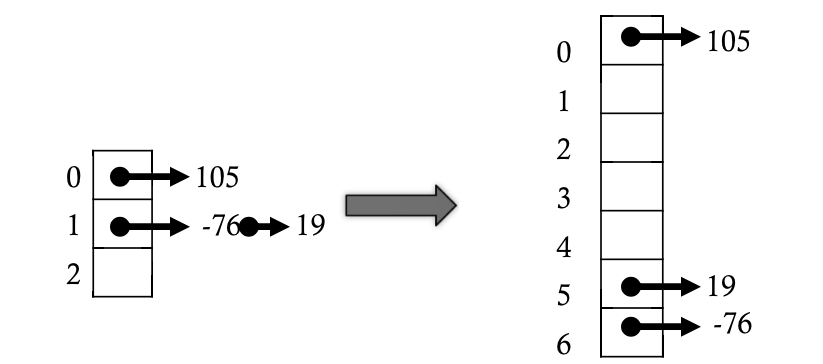
\includegraphics[width=0.5\textwidth]{images/1.png}    
\end{center}

\subsection*{Hash Table Overview}
\begin{itemize}
    \item \textit{Separate Chaining}: expand the single array entry into a linked list
    \begin{itemize}
        \item Compute the integer hash code from the element
        \item Bound the values to allow us to easily calculate the index
        \item Find the list to operate on
    \end{itemize}
    \item \mintinline{java}{.add(T t)}: put \mintinline{java}{t} in the hash-table
    \begin{itemize}
        \item Add the item with \mintinline{java}{list.add(t);}
        \item Rehash the entire table if the load is too high
    \end{itemize}
    \item \mintinline{java}{.has(T t)}: check if the element is already in the list
    \begin{itemize}
        \item \mintinline{java}{return list.contains(t);}
    \end{itemize}
    \item \mintinline{java}{.remove(T t)}: delete the element from the list
    \begin{itemize}
        \item \mintinline{java}{list.remove(t);}
    \end{itemize}
\end{itemize}

\subsection*{Big-O Analysis}
\begin{center}
    \begin{tabular}{lcccr}
        \toprule
        & \mintinline{java}{.add()}* & \mintinline{java}{.has()} & \mintinline{java}{.remove()} & iteration \\ \midrule
        Best & $O(1)$ & $O(1)$ & $O(1)$ & $O(n+m)$ \\
        Average & $O(n/m)$ & $O(n/m)$ & $O(n/m)$ & $O(n+m)$ \\
        Worst & $O(n)$ & $O(n)$ & $O(n)$ & $O(n+m)$ \\ \bottomrule
    \end{tabular}
\end{center}
\begin{itemize}
    \item Hash table with separate chaining (*assuming no duplicates are allowed, and not considering rehashing overhead)
    \begin{itemize}
        \item The load is $n/m$
        \item $n$ is the number of values in the hash-table
        \item $m$ is the number of entries (array capacity)
    \end{itemize}
\end{itemize}

\subsection*{Separate Chaining is Viable in Practice}
\begin{itemize}
    \item Simple to implement
    \begin{itemize}
        \item Weiss Figure 20.20
    \end{itemize}
    \item Reasonably efficient
    \item A ``chain'' can be implemented as a different data structure
    \begin{itemize}
        \item We can use trees, an \mintinline{java}{ArrayList}, or others
        \item Binary search trees can be used if there are no duplicates allowed
    \end{itemize}
    \item Java's built-in hash tables use separate chaining
    \begin{itemize}
        \item \mintinline{java}{java.util.HashSet}, \mintinline{java}{java.util.HashMap}, and \mintinline{java}{java.util.Hashtable} all use separate chaining
        \item \mintinline{java}{java.util.HashMap} uses red-black trees when the number of values in one chain is more than eight
    \end{itemize}
\end{itemize}

\subsection*{Hash Code Review}
\begin{itemize}
    \item We define a hash function to map any object to a manageable integer as its hash code
    \begin{itemize}
        \item \mintinline{java}{.hashCode()} defined in \mintinline{java}{java.lang.Object}
    \end{itemize}
    \item Hash contract: objects that are identical must have the same hash code
    \item We need hash functions that are easy to compute and distribute well
    \item Java provides implementations for built-in types
\end{itemize}


\subsection*{Hash Code in Java}
\begin{itemize}
    \item Built in for boxed and container types (\mintinline{java}{Integer}, \mintinline{java}{Integer[]}, etc.)
    \item The output is a 32-bit integer
    \item Straightforward for types with a size of no more than 32 bits
    \begin{itemize}
        \item If that's true, it's trivial to map every unique value to a different integer
        \begin{itemize}
            \item This works for our \mintinline{java}{Integer}, \mintinline{java}{Boolean}, and \mintinline{java}{Character} types
        \end{itemize}
        \item Types with a larger size use the following trick
        \begin{itemize}
            \item Exclusive OR the two halves to reduce the reference from 8 bytes to 4 bytes
            \begin{itemize}
                \item \mintinline{java}{(int) (this.longValue() ^ (this.longValue() >>> 32))} (that's the logical shift right)
            \end{itemize}
        \end{itemize}
    \end{itemize}
\end{itemize}

\subsection*{Aggregate Type: String}
\begin{itemize}
    \item The hash code for a string object is computed by taking the $\beta$-expansion where the most-significant-place is the ASCII value of the first index of the string (and the base is 31)
    \begin{itemize}
        \item It follows then that the hash value of the empty string is zero
    \end{itemize}
    \item Discussion
    \begin{itemize}
        \item Is 31 special?
        \begin{itemize}
            \item ``According to Joshua Bloch's Effective Java (a book that can't be recommended enough, and which I bought thanks to continual mentions on stackoverflow):
            
            \begin{itemize}
                \item[] The value 31 was chosen because it is an odd prime. If it were even and the multiplication overflowed, information would be lost, as multiplication by 2 is equivalent to shifting. The advantage of using a prime is less clear, but it is traditional. A nice property of 31 is that the multiplication can be replaced by a shift and a subtraction for better performance:
            
                \mintinline{java}{31 * i == (i << 5) - i}.
            
                Modern VMs do this sort of optimization automatically.
            \end{itemize}
            
            \textit{(from Chapter 3, Item 9: Always override hashcode when you override equals, page 48)}"

            (Taken from \url{https://stackoverflow.com/a/299748}) 
            
            \item Getting more into the math, using a prime number for the modulo is important because (I think -- my abstract algebra is weak to non-existent) the Integers modulo a prime number are a field, whereas with other non-prime numbers they are only a ring.
            
            This is also typically why we use addition and multiplication -- the integers under modulo are closed under these operations.
            
            An added benefit of using a prime number for both hash function and the modulo is that they are \textit{highly} unlikely to share factors in common. (Common factors in the hash function and the modulo result in more collisions.)
            
            \item ``You can read Bloch's original reasoning under ``Comments" in \url{http://bugs.java.com/bugdatabase/view_bug.do?bug_id=4045622}. He investigated the performance of different hash functions in regards to the resulting "average chain size" in a hash table. \mintinline{java}{P(31)} was one of the common functions during that time which he found in K\&R's book (but even Kernighan and Ritchie couldn't remember where it came from). In the end he basically had to choose one and so he took \mintinline{java}{P(31)} since it seemed to perform well enough. Even though \mintinline{java}{P(33)} was not really worse and multiplication by 33 is equally fast to calculate (just a shift by 5 and an addition), he opted for 31 since 33 is not a prime:

            \begin{itemize}
                \item[] Of the remaining four, I'd probably select \mintinline{java}{P(31)}, as it's the cheapest to calculate on a RISC machine (because 31 is the difference of two powers of two). \mintinline{java}{P(33)} is similarly cheap to calculate, but it's performance is marginally worse, and 33 is composite, which makes me a bit nervous.
            \end{itemize}

            So the reasoning was not as rational as many of the answers here seem to imply. But we're all good in coming up with rational reasons after gut decisions (and even Bloch might be prone to that)."
            
            (Taken from \url{https://stackoverflow.com/a/35304979})
        \end{itemize}
        
        \item \textbf{Can you write code to compute the hash code faster instead of following the formula strictly?}
        \begin{itemize}
            \item I mean, probably. I like the trick with exclusive or for hashing references (which are typically 64 bits on most modern machines).
        \end{itemize}
    \end{itemize}
\end{itemize}

\subsection*{Polynomial Hash Code}
\begin{itemize}
    \item String uses a polynomial hash code
    $$ a_0 \beta^{n-1} + \dots + a_{n-1} \beta^0$$
    \begin{itemize}
        \item Java uses $\beta=31$ for strings
    \end{itemize}
    \item Optimize
    \begin{itemize}
        \item We can regroup a polynomial of any degree and reduce the power calculation to multiplication
        \item Example of regrouping a degree 3 polynomial so that we don't have to use exponentiation:
        $$ a_0 \beta^{3} + a_1 \beta^2 + a_2 \beta + a_3$$
        becomes
        $$(((a_0 \beta)\beta + a_1)\beta + a_2)\beta + a_3$$
    \end{itemize}
\end{itemize}

\subsection*{Aggregate Type Hashing}
\begin{itemize}
    \item Other aggregate types
    \begin{itemize}
        \item Use the String approach: create a polynomial has code using each of the elements, computing each element's hash individually
    \end{itemize}
    \item The poor man's strategy: \mintinline{java}{x.toString().hashCode()}
\end{itemize}

\subsection*{Object Hash Code Example}
\begin{minted}{java}
// Composite hashCode from all attributes
public class Student {
    private String name;
    private int age;
    private double grade;
    ...
    // Note: Default is memory address, not proper hashCode!!!
    @Override
    public int hashCode( ) {
        int hash = 17; // pick prime constants
        hash = 31 * hash + name.hashCode();
        hash = 31 * hash + ((Integer) age).hashCode();
        hash = 31 * hash + ((Double) grade).hashCode();
        return hash;
    } 
} 
\end{minted}

\end{document}